% Options for packages loaded elsewhere
\PassOptionsToPackage{unicode}{hyperref}
\PassOptionsToPackage{hyphens}{url}
%
\documentclass[
  12pt,
  a4paper,
  DIV=11,
  numbers=noendperiod]{scrreprt}

\usepackage{amsmath,amssymb}
\usepackage{setspace}
\usepackage{iftex}
\ifPDFTeX
  \usepackage[T1]{fontenc}
  \usepackage[utf8]{inputenc}
  \usepackage{textcomp} % provide euro and other symbols
\else % if luatex or xetex
  \usepackage{unicode-math}
  \defaultfontfeatures{Scale=MatchLowercase}
  \defaultfontfeatures[\rmfamily]{Ligatures=TeX,Scale=1}
\fi
\usepackage{lmodern}
\ifPDFTeX\else  
    % xetex/luatex font selection
\fi
% Use upquote if available, for straight quotes in verbatim environments
\IfFileExists{upquote.sty}{\usepackage{upquote}}{}
\IfFileExists{microtype.sty}{% use microtype if available
  \usepackage[]{microtype}
  \UseMicrotypeSet[protrusion]{basicmath} % disable protrusion for tt fonts
}{}
\usepackage{xcolor}
\setlength{\emergencystretch}{3em} % prevent overfull lines
\setcounter{secnumdepth}{5}
% Make \paragraph and \subparagraph free-standing
\ifx\paragraph\undefined\else
  \let\oldparagraph\paragraph
  \renewcommand{\paragraph}[1]{\oldparagraph{#1}\mbox{}}
\fi
\ifx\subparagraph\undefined\else
  \let\oldsubparagraph\subparagraph
  \renewcommand{\subparagraph}[1]{\oldsubparagraph{#1}\mbox{}}
\fi


\providecommand{\tightlist}{%
  \setlength{\itemsep}{0pt}\setlength{\parskip}{0pt}}\usepackage{longtable,booktabs,array}
\usepackage{calc} % for calculating minipage widths
% Correct order of tables after \paragraph or \subparagraph
\usepackage{etoolbox}
\makeatletter
\patchcmd\longtable{\par}{\if@noskipsec\mbox{}\fi\par}{}{}
\makeatother
% Allow footnotes in longtable head/foot
\IfFileExists{footnotehyper.sty}{\usepackage{footnotehyper}}{\usepackage{footnote}}
\makesavenoteenv{longtable}
\usepackage{graphicx}
\makeatletter
\def\maxwidth{\ifdim\Gin@nat@width>\linewidth\linewidth\else\Gin@nat@width\fi}
\def\maxheight{\ifdim\Gin@nat@height>\textheight\textheight\else\Gin@nat@height\fi}
\makeatother
% Scale images if necessary, so that they will not overflow the page
% margins by default, and it is still possible to overwrite the defaults
% using explicit options in \includegraphics[width, height, ...]{}
\setkeys{Gin}{width=\maxwidth,height=\maxheight,keepaspectratio}
% Set default figure placement to htbp
\makeatletter
\def\fps@figure{htbp}
\makeatother

\usepackage{indentfirst}
\usepackage{float}
\floatplacement{figure}{H}
\IfFileExists{plex-otf.sty}{
  %% Full TeXlive
  \usepackage[
    % math,
    RM={Scale=0.94},SS={Scale=0.94},SScon={Scale=0.94},TT={Scale=MatchLowercase,FakeStretch=0.9},
    DefaultFeatures={Ligatures=Common}
  ]{plex-otf}
  % \usepackage[Scale=MatchUppercase]{juliamono}
}{
  %% TinyTeX
  \usepackage{libertine}
}
\KOMAoption{captions}{tableheading}
\makeatletter
\@ifpackageloaded{caption}{}{\usepackage{caption}}
\AtBeginDocument{%
\ifdefined\contentsname
  \renewcommand*\contentsname{Содержание}
\else
  \newcommand\contentsname{Содержание}
\fi
\ifdefined\listfigurename
  \renewcommand*\listfigurename{Список иллюстраций}
\else
  \newcommand\listfigurename{Список иллюстраций}
\fi
\ifdefined\listtablename
  \renewcommand*\listtablename{Список таблиц}
\else
  \newcommand\listtablename{Список таблиц}
\fi
\ifdefined\figurename
  \renewcommand*\figurename{Рисунок}
\else
  \newcommand\figurename{Рисунок}
\fi
\ifdefined\tablename
  \renewcommand*\tablename{Таблица}
\else
  \newcommand\tablename{Таблица}
\fi
}
\@ifpackageloaded{float}{}{\usepackage{float}}
\floatstyle{ruled}
\@ifundefined{c@chapter}{\newfloat{codelisting}{h}{lop}}{\newfloat{codelisting}{h}{lop}[chapter]}
\floatname{codelisting}{Список}
\newcommand*\listoflistings{\listof{codelisting}{Листинги}}
\makeatother
\makeatletter
\makeatother
\makeatletter
\@ifpackageloaded{caption}{}{\usepackage{caption}}
\@ifpackageloaded{subcaption}{}{\usepackage{subcaption}}
\makeatother
\ifLuaTeX
\usepackage[bidi=basic]{babel}
\else
\usepackage[bidi=default]{babel}
\fi
\babelprovide[main,import]{russian}
\babelprovide[import]{english}
% get rid of language-specific shorthands (see #6817):
\let\LanguageShortHands\languageshorthands
\def\languageshorthands#1{}
\ifLuaTeX
  \usepackage{selnolig}  % disable illegal ligatures
\fi
\usepackage[style=gost-numeric,backend=biber,langhook=extras,autolang=other*]{biblatex}
\addbibresource{bib/cite.bib}
\usepackage{csquotes}
\usepackage{bookmark}

\IfFileExists{xurl.sty}{\usepackage{xurl}}{} % add URL line breaks if available
\urlstyle{same} % disable monospaced font for URLs
\hypersetup{
  pdftitle={Отчет по лабораторной работе 3},
  pdfauthor={Зорова Ульяна Владимировна},
  pdflang={ru-RU},
  pdfkeywords={лабораторная работа, шаблон, Markdown, Pandoc},
  hidelinks,
  pdfcreator={LaTeX via pandoc}}

\title{Отчет по лабораторной работе 3}
\usepackage{etoolbox}
\makeatletter
\providecommand{\subtitle}[1]{% add subtitle to \maketitle
  \apptocmd{\@title}{\par {\large #1 \par}}{}{}
}
\makeatother
\subtitle{Язык разметки Markdown}
\author{Зорова Ульяна Владимировна}
\date{}

\begin{document}
\maketitle
\begin{abstract}
В данном документе приведены итоги выполнения лабораторной работы 3,
направленной на изучение процесса формирования отчетов с применением
облегченного языка разметки Markdown.
\end{abstract}

\renewcommand*\contentsname{Содержание}
{
\setcounter{tocdepth}{1}
\tableofcontents
}
\listoffigures
\listoftables
\setstretch{1.5}
\chapter{Цель
работы}\label{ux446ux435ux43bux44c-ux440ux430ux431ux43eux442ux44b}

Изучить и применить на практике процедуру оформления отчетов с помощью
облегченного языка разметки Markdown.

\chapter{Выполнение лабораторной
работы}\label{ux432ux44bux43fux43eux43bux43dux435ux43dux438ux435-ux43bux430ux431ux43eux440ux430ux442ux43eux440ux43dux43eux439-ux440ux430ux431ux43eux442ux44b}

Я запустила терминал, переместилась в каталог учебного курса (созданный
на этапе второй лабораторной работы) и обновила локальную копию
репозитория с помощью команды git pull (Рисунок~\ref{fig-1})

\begin{figure}

\centering{

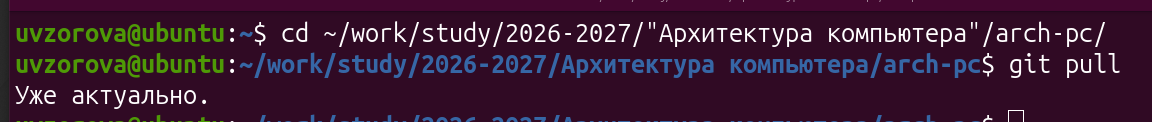
\includegraphics[width=0.8\textwidth,height=\textheight]{image/1.png}

}

\caption{\label{fig-1}переход в каталог курса и обновление репозитория}

\end{figure}%

Затем я перешла в папку с отчетом по третьей лабораторной работе и
запустила компиляцию шаблона, используя Makefile и команду make
(Рисунок~\ref{fig-2})

\begin{figure}

\centering{

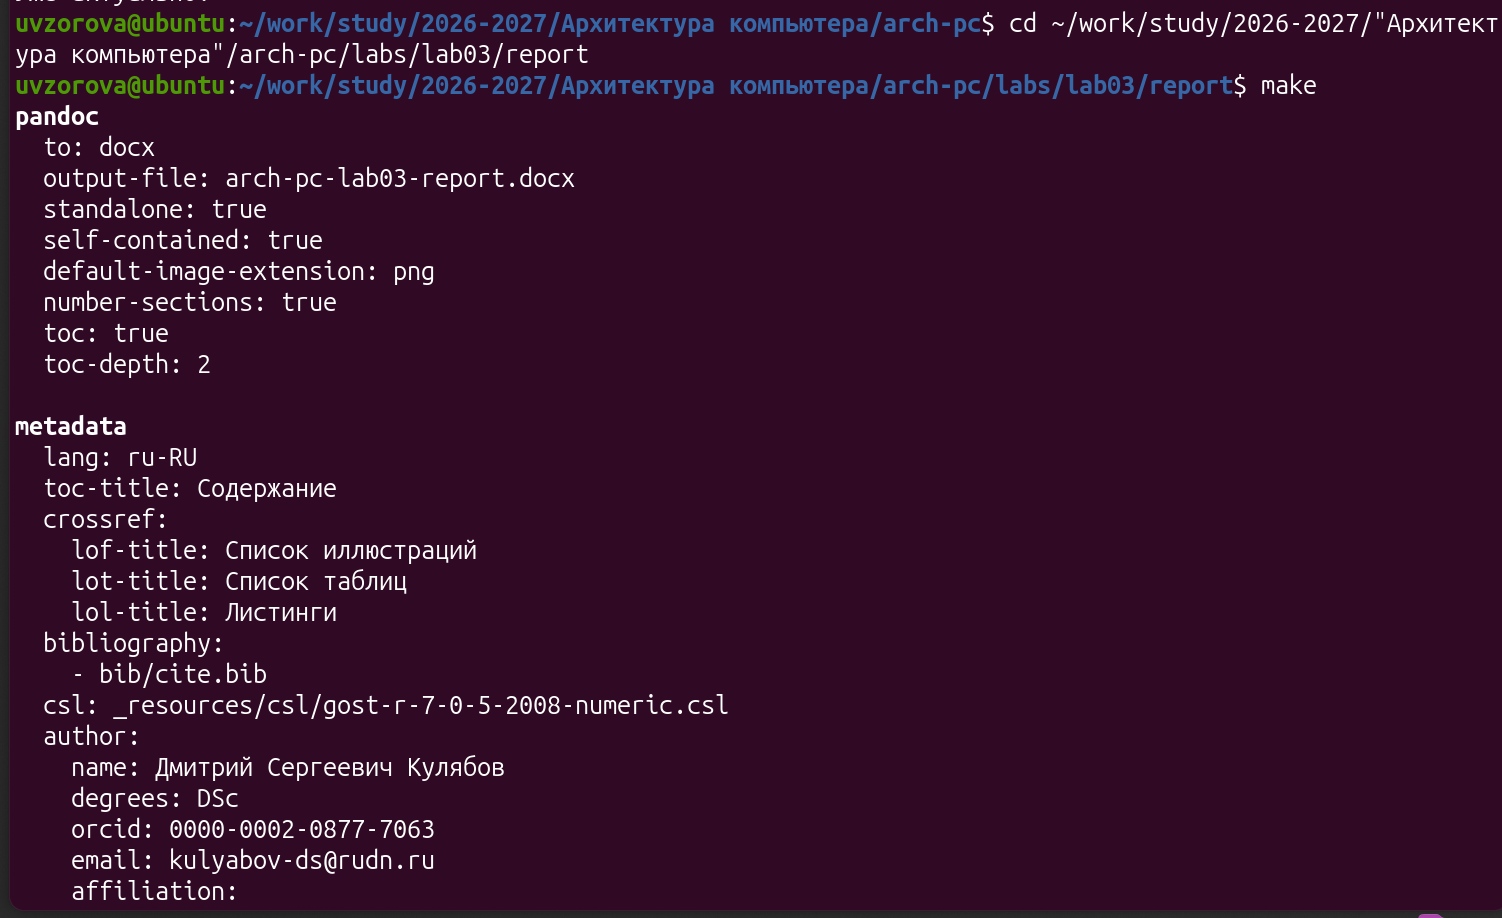
\includegraphics[width=0.8\textwidth,height=\textheight]{image/2.png}

}

\caption{\label{fig-2}переход в каталог labs/lab03/report и компиляция
шаблона}

\end{figure}%

В результате выполнения команды были созданы файлы
arch-pc-lab03-report.docx и arch-pc-lab03-report.pdf
(Рисунок~\ref{fig-3})

\begin{figure}

\centering{

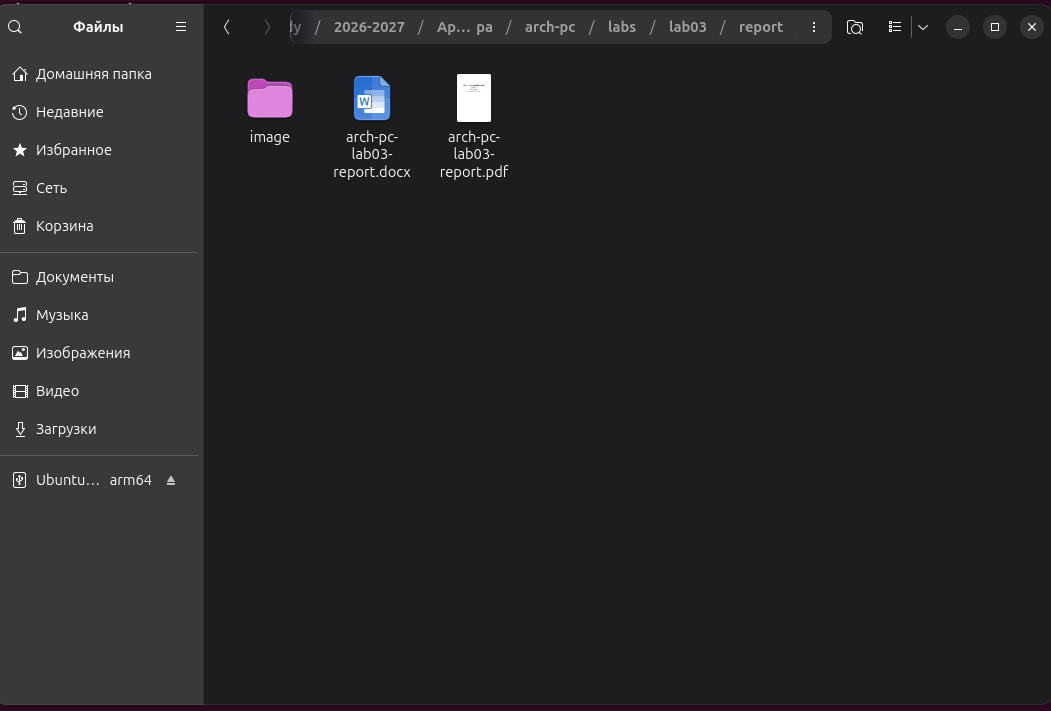
\includegraphics[width=0.8\textwidth,height=\textheight]{image/3.png}

}

\caption{\label{fig-3}сгенерированные файлы в файловом менеджере}

\end{figure}%

Затем я удалила эти сгенерированные файлы с помощью команды make clean
(Рисунок~\ref{fig-4})

\begin{figure}

\centering{

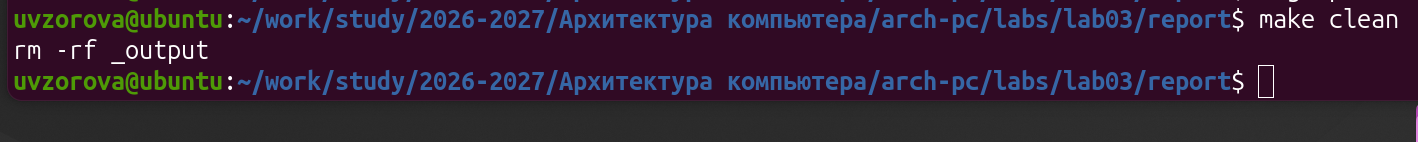
\includegraphics[width=0.8\textwidth,height=\textheight]{image/4.png}

}

\caption{\label{fig-4}удаление файлов}

\end{figure}%

После этого я открыла исходный файл arch-pc-lab03-report.qmd и детально
изучила его структуру (Рисунок~\ref{fig-5})

\begin{figure}

\centering{

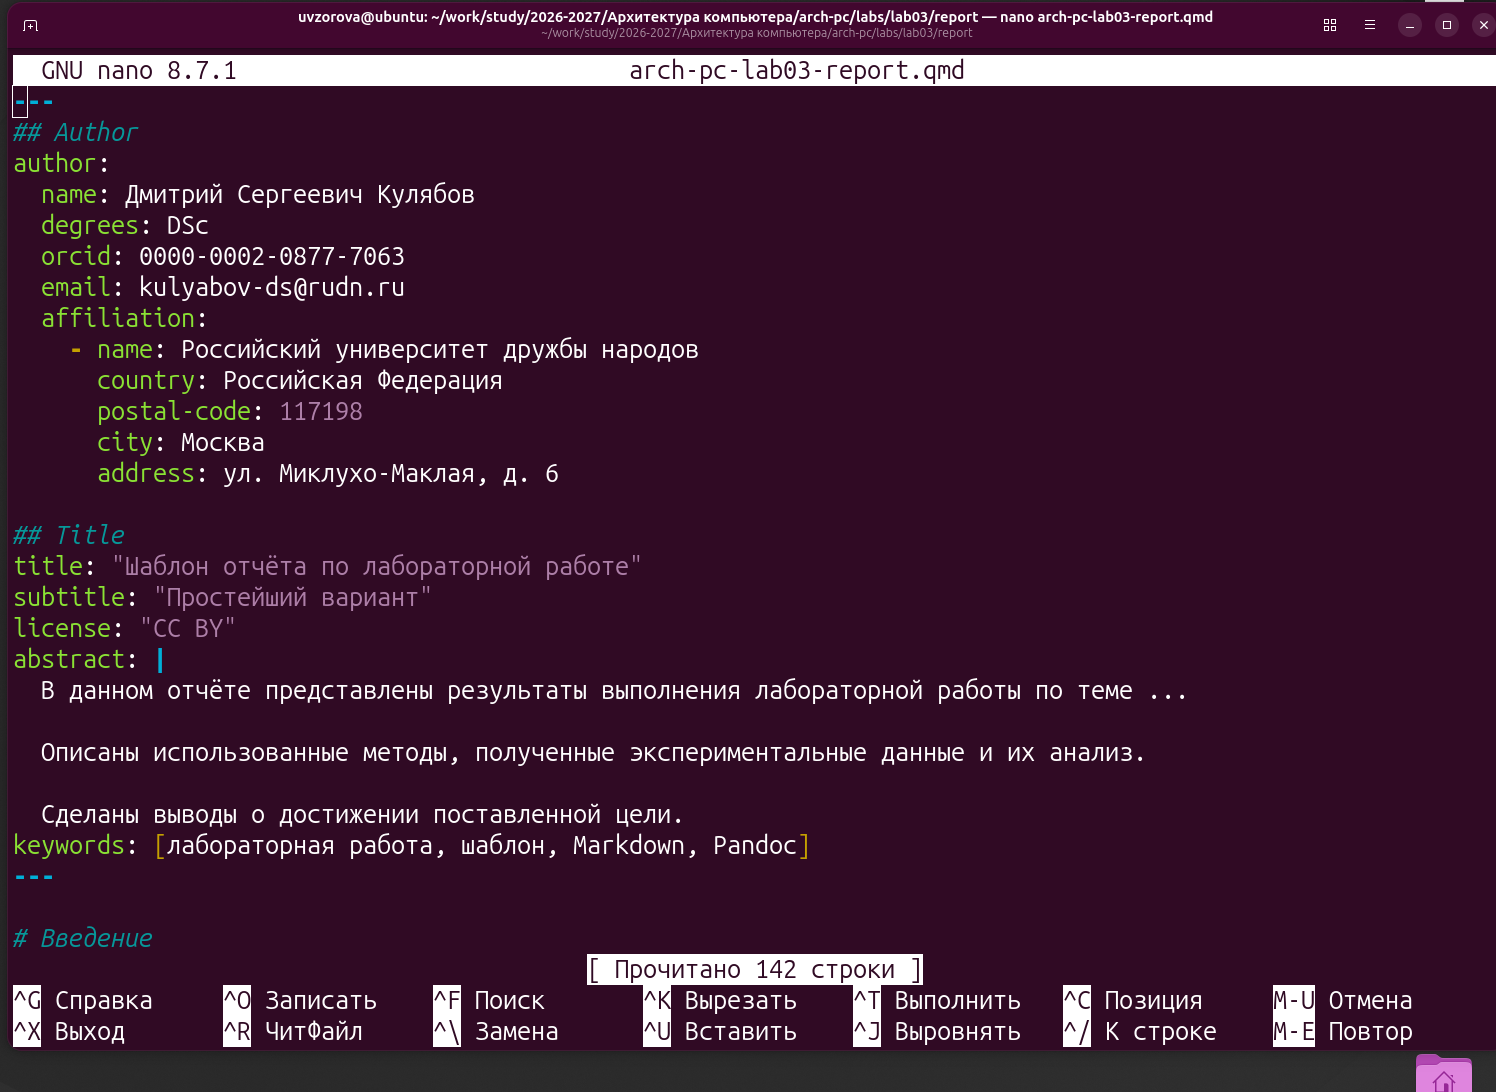
\includegraphics[width=0.8\textwidth,height=\textheight]{image/5.png}

}

\caption{\label{fig-5}файл arch-pc-lab03.qmd, открытый в редакторе}

\end{figure}%

Опираясь на изученный шаблон arch-pc-lab03-report.qmd, я сформировала
собственный отчет по лабораторной работе 3. С помощью команды make я
заново сгенерировала файлы arch-pc-lab03-report.docx и
arch-pc-lab03-report.pdf, но уже с моим текстом (Рисунок~\ref{fig-6})

\begin{figure}

\centering{

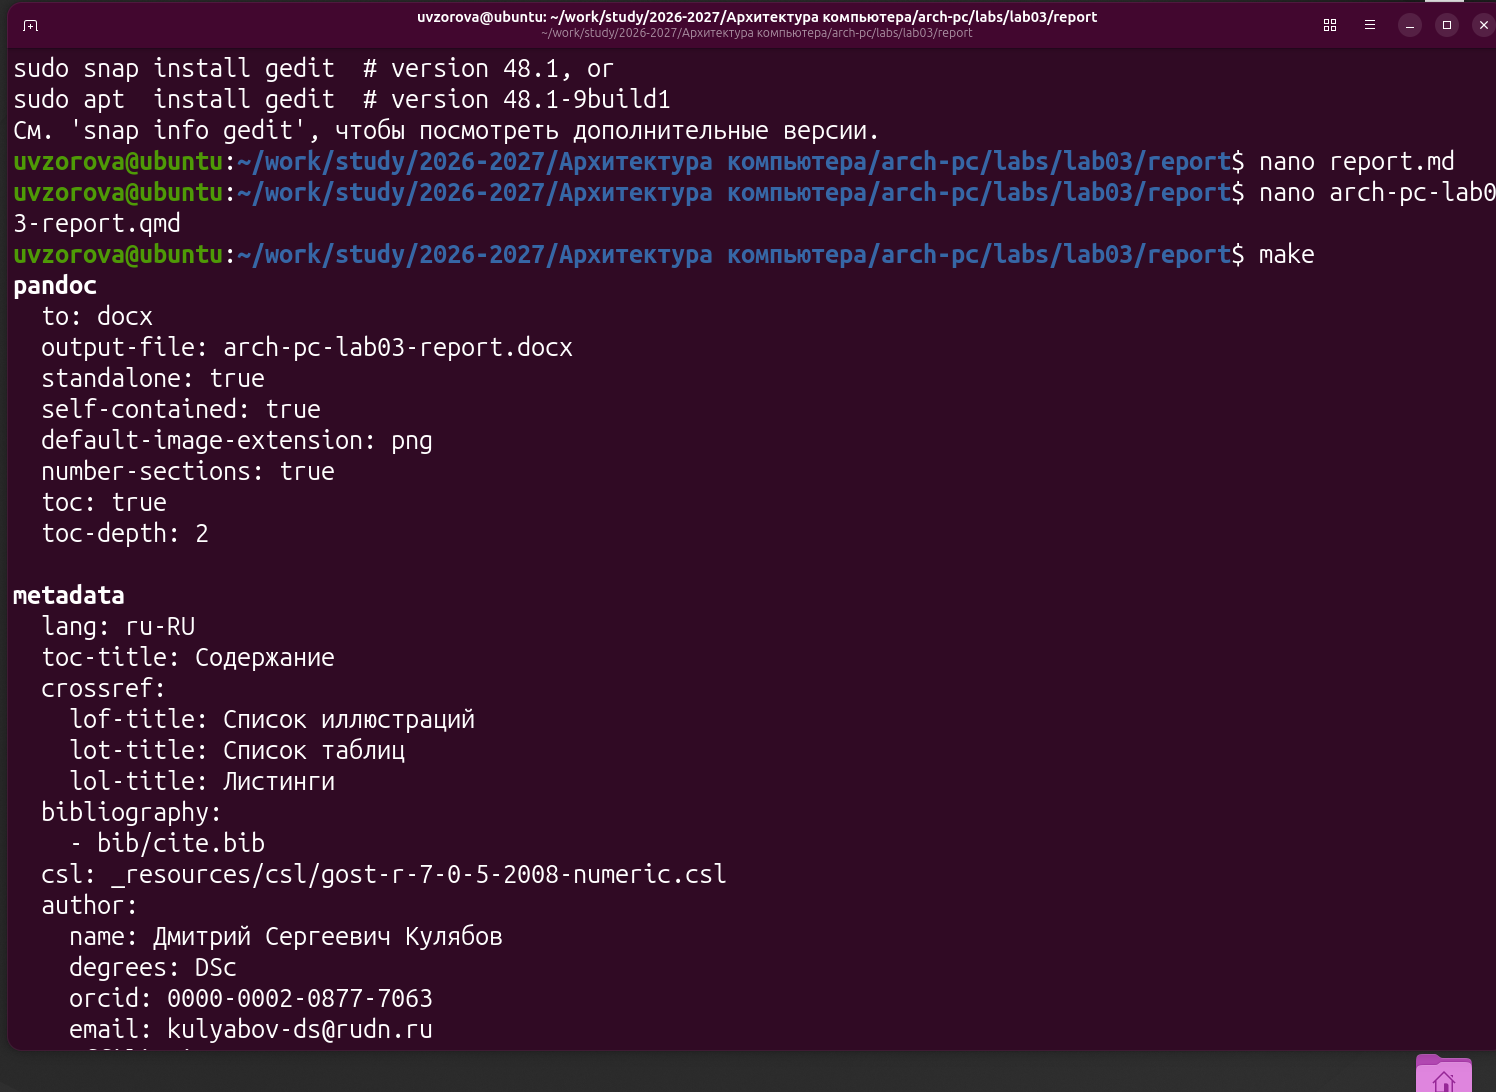
\includegraphics[width=0.8\textwidth,height=\textheight]{image/6.png}

}

\caption{\label{fig-6}повторная генерация файлов}

\end{figure}%

Далее я загрузила готовые файлы на gitverse. Для этого в терминале были
последовательно введены команды git add ., git commit -am
\enquote*{feat(main): add files lab-3}, git push

\chapter{Выполнение самостоятельной
работы}\label{ux432ux44bux43fux43eux43bux43dux435ux43dux438ux435-ux441ux430ux43cux43eux441ux442ux43eux44fux442ux435ux43bux44cux43dux43eux439-ux440ux430ux431ux43eux442ux44b}

В каталоге labs/lab02/report я создала отчет по второй лабораторной
работе в трех форматах: .pdf, .docx, .md, после чего также загрузила их
на gitverse (Рисунок~\ref{fig-7})

\begin{figure}

\centering{

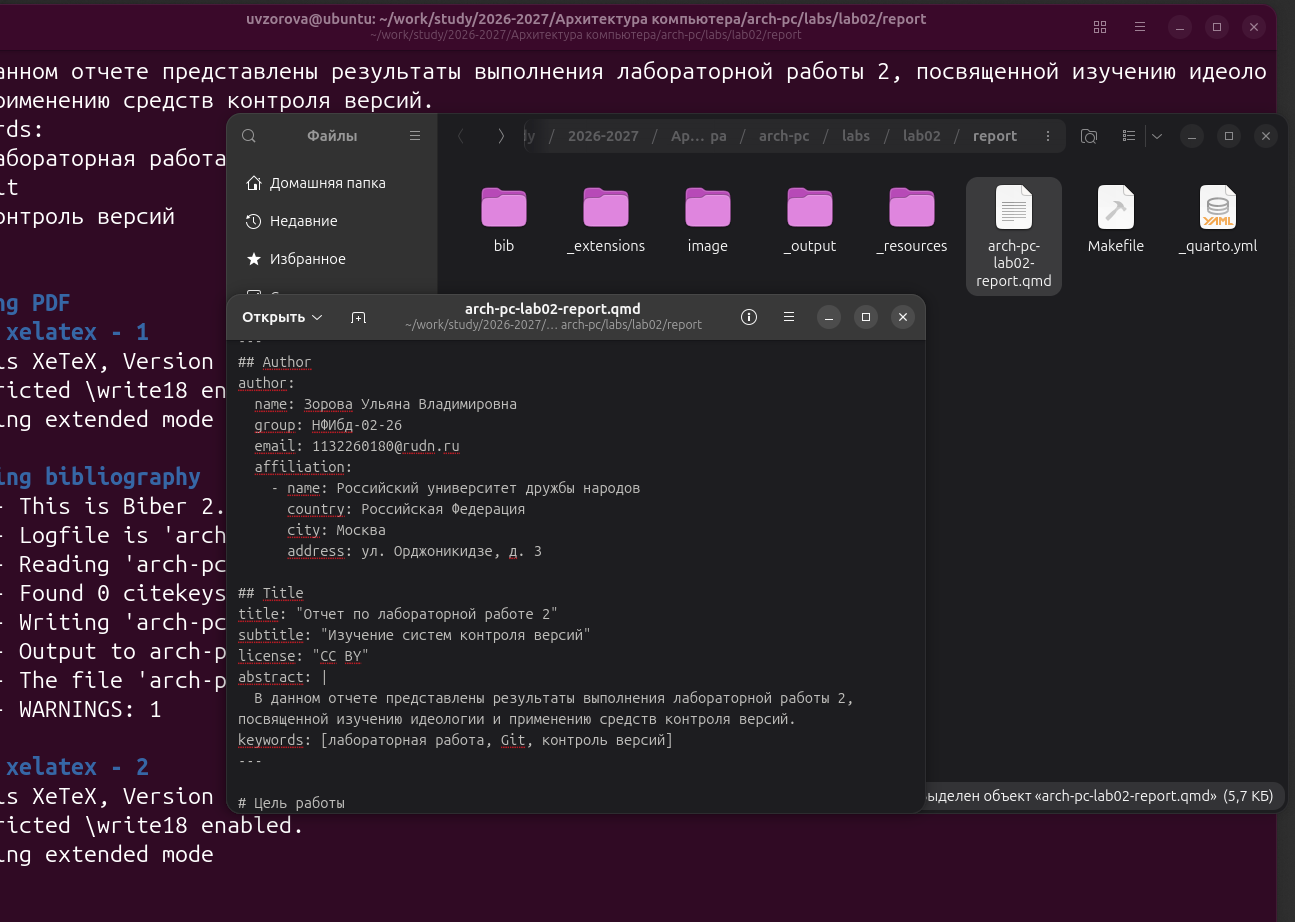
\includegraphics[width=0.8\textwidth,height=\textheight]{image/7.png}

}

\caption{\label{fig-7}процесс создания отчета по второй лабораторной с
помощью Markdown}

\end{figure}%

Ссылка на мой репозиторий:
\href{https://github.com/UVZorova/study_2026-2027_arh-pc}{Gitverse
Зорова Ульяна}

\chapter{Вывод}\label{ux432ux44bux432ux43eux434}

В ходе выполнения работы я освоила процедуры оформления отчетов с
использованием легковесного языка разметки Markdown.


\printbibliography


\end{document}
